\begin{frame}{Allgemeines}{Baumstrukturen (Vgl. \cite{fahr:list})}
	\begin{itemize}
		\item Unterscheiden sich von den bisherigen Strukturen
		\item Bisher hatte jedes Element einer Datenstruktur immer einen "`Nachfolger"'
		\item ...und einen Vorgänger
		\item Bäume können jedoch mehrere "`Nachfolger"' haben
		\begin{itemize}
			\item Man spricht in der Regel von \textbf{Knoten}
			\item Es gibt genau einen Knoten im Baum, der keinen Eingang ("`Vorgänger"') besitzt
			\begin{itemize}
				\item Dies ist der \textbf{Wurzelknoten} des Baumes
			\end{itemize}
			\item Alle anderen Knoten haben genau einen Eingang
		\end{itemize}
		\item In der Regel beschäftigt man sich hauptsächlich mit \textit{Binärbäumen}
	\end{itemize}
\end{frame}

\begin{frame}{Bäume}{Graphentheoretische Definition (Vgl. \cite{fahr:list})}
	\vfill
	\begin{alertblock}{Graphentheoretische Definition}
	Ein Baum ist ein endlicher, schwach zusammenhängender gerichteter Graph, für dessen Knotenpunkte gilt:
	\begin{enumerate}
		\item Es gibt genau einen Knoten, der keinen Eingang hat (Wurzel des Baumes)
		\item Alle übrigen Knotenpunkte haben genau einen Eingang.
	\end{enumerate}
	\end{alertblock}
	\vfill
\end{frame}

\begin{frame}{Allgemeines}{Rekursive Definition (Vgl. \cite{fahr:list})}
	\vfill
	\begin{alertblock}{Rekursive Definition(Binärbaum)}
	Eine Baumstruktur vom Grundtyp T ist:
	\begin{enumerate}
		\item Eine leere Struktur
		\item Ein Knoten vom Typ T mit genau zwei disjunkten Teilbäume vom Grundtyp T
	\end{enumerate}
	\end{alertblock}
	\vfill
\end{frame}

\begin{frame}{Allgemeines}{Struktur der Knoten im Baum (Vgl. \cite{fahr:list})}
	\begin{itemize}
		\item Grundsätzlich besteht ein Knoten(Im Binärbaum) aus drei Elementen
		\begin{itemize}
			\item Einem Schlüssel (=Datenwert) für den Knoten
			\item Einen linken Teilbaum
			\item Einen rechten Teilbaum
		\end{itemize}
	\end{itemize}
\end{frame}

\begin{frame}{Eigenschaften}{Vollständige Binärbäume (Vgl. \cite{fahr:list})}
	\vfill
	\begin{alertblock}{Vollständige Binärbäume}
	In einem Binärbaum kann jede Ebene maximal $2^{(Tiefe-1)}$ Knoten besitzen. Ein Binärbaum ist dann vollständig ausgeglichen, wenn auf jeder Ebene, mit Ausnahme der letzten, genau diese
	$2^{(Tiefe-1)}$ Knoten existieren und die Knoten auf der letzten Ebene soweit links wie möglich stehen
	\end{alertblock}
	\vfill
\end{frame}

\begin{frame}{Eigenschaften}{Suchbäume (Vgl. \cite{fahr:list})}
	\vfill
	\begin{alertblock}{Suchbaum}
	Wenn für alle Knoten K eines Baumes gilt, dass...
	\begin{enumerate}
		\item ...alle Schlüssel im linken Teilbaum von K kleiner...
		\item ...alle Schlüssel im rechten Teilbaum von K größer...
	\end{enumerate}
	... als der Schlüssel des Knotens K sind, so handelt es sich um einen Suchbaum
	\end{alertblock}
	\vfill
\end{frame}

\begin{frame}{Grundoperationen}{In Binärbäumen}
	\begin{itemize}
		\item Zur Vereinfachung betrachten wir für Binärbäume (Suchbäume) folgende Operationen:
		\begin{itemize}
			\item Einfügen von Elementen
			\item Entfernen von Elementen
			\item Bestimmen der Anzahl von Elementen
		\end{itemize}
		\item Grundoperationen basieren fast immer auf rekursivem Aufruf auf den Teilbäumen!
	\end{itemize}
\end{frame}

\begin{frame}{Grundoperationen}{Einfügen von Elementen (Vgl. \cite{fahr:list})}
	\begin{itemize}
		\item Für das Einfügen eines Elements $X$ in einen Baum $B$ werden vier Fälle unterschieden:
		\begin{itemize}
			\item Ist $B$ leer, so ist das Ergebnis der Baum mit dem Schlüssel $X$
			\item Ist $X$ identisch mit dem Schlüssel von $B$ so ist $X$ bereits im Baum und wird nicht hinzugefügt
			\item Ist $X$ kleiner als der Schlüssel von $B$ so füge $X$ im linken Teilbaum ein
			\item Ist $X$ größer als der Schlüssel von $B$ so füge $X$ im rechten Teilbaum ein
		\end{itemize}
	\end{itemize}
\end{frame}

\begin{frame}{Grundoperationen}{Entfernen aus Suchbäumen}
\begin{itemize}
	\item Beim Entfernen eines Elements mit dem Schlüssel $X$ können vier Fälle auftreten:
	\begin{itemize}
		\item Der Baum enthält $X$ nicht - Fertig.
		\item Der Knoten mit dem Schlüssel $X$ hat keinen Nachfolger - $X$ wird entfernt, Fertig.
		\item Der Knoten mit dem Schlüssel $X$ hat genau einen Nachfolger
		\item Der Knoten mit dem Schlüssel $X$ hat genau zwei Nachfolger
	\end{itemize}
\end{itemize}
\end{frame}

\begin{frame}{Entfernen}{$X$ hat einen Nachfolger (Vgl. \cite{tree1}, \cite{tree2})}
	\begin{itemize}
		\item Simpler Fall
		\item Hier "`rutscht"' der Nachfolger (Gesamter Teilbaum) einfach an die Stelle des zu entfernenden Elements
		\item Keine weiteren Operationen - Fertig.
	\end{itemize}
\end{frame}

\begin{frame}{Entfernen}{$X$ hat zwei Nachfolger (Vgl. \cite{tree1}, \cite{tree2})}
	\begin{itemize}
		\item Problematik: Welcher Nachfolger tritt an die Stelle von $X$
		\item ...damit die Suchbaumbedingung bestehen bleibt?
		\item Suchen des sogenannten \textbf{in-order Nachbarn} $N$ von $X$
		\begin{itemize}
			\item Ist das jeweils nächstgrößere bzw. -kleinere Element an $X$
			\item Also das kleinste ("`linkeste"') Element des rechten Teilbaums
			\item Oder größtes ("`rechteste"') Element des linken Teilbaums
		\end{itemize}
		\item $N$ tritt an die Stelle von $X$
		\item Teilbäume von $X$ bleiben (beinahe) unervändert
		\begin{itemize}
			\item Außer natürlich, dass $N$ aus dem Teilbaum entfernt wird
		\end{itemize}
	\end{itemize}
\end{frame}

\begin{frame}{Grundoperationen}{Bestimmen der Anzahl der Elemente}
	\begin{itemize}
		\item Wie in allen Strukturen kann die Anzahl der Elemente natürlich manuell verwaltet werden
		\item Allerdings ist das Zählen auch über eine rekursive Definition möglich
		\item Hierbei Unterscheidung zwischen zwei Fällen:
		\begin{itemize}
			\item Ist der Baum $B$ die leere Struktur, so ist die Größe $0$
			\item Sonst gilt: $size(B)=size(L)+size(R)+1$, wobei $L$ und $R$ den linken bzw. rechten Teilbaum bezeichnen
		\end{itemize}
	\end{itemize}
\end{frame}

\begin{frame}{Ausgeglichenheit}{Das Ying und Yang von Bäumen}
	\begin{itemize}
		\item Bisher können unsere (Teil-)Bäume verschiedene Tiefen haben
		\item Dies ist jedoch nicht optimal für z.B. Suchalgorithmen
		\item Die maximale Suchzeit lässt sich so nur schwer abschätzen
		\item Außerdem ist die durchschnittliche Suchzeit meist höher
		\item Daher:
		\begin{itemize}
			\item Definition eines Ausgeglichenheitskriteriums
			\item Dadurch Tiefe der Teilbäume ähnlich
			\item Führt zu besserer Performance bei Suchbäumen
		\end{itemize}
	\end{itemize}
\end{frame}

\begin{frame}{AVL Bäume}{Definition (Vgl. \cite{fahr:list}, \cite{mutzel:avl})}
	\vfill
	\begin{alertblock}{Ausgeglichenheit nach AVL-Bedingung}
	Ein Baum ist dann ausgeglichen, wenn sich für jeden Knoten die Höhe der zugehörigen Teilbäume um
	höchstens 1 unterscheidet.
	\end{alertblock}
	\vfill
\end{frame}

\begin{frame}{AVL Bäume}{Visualisiert}
	\begin{figure}
	\centering
	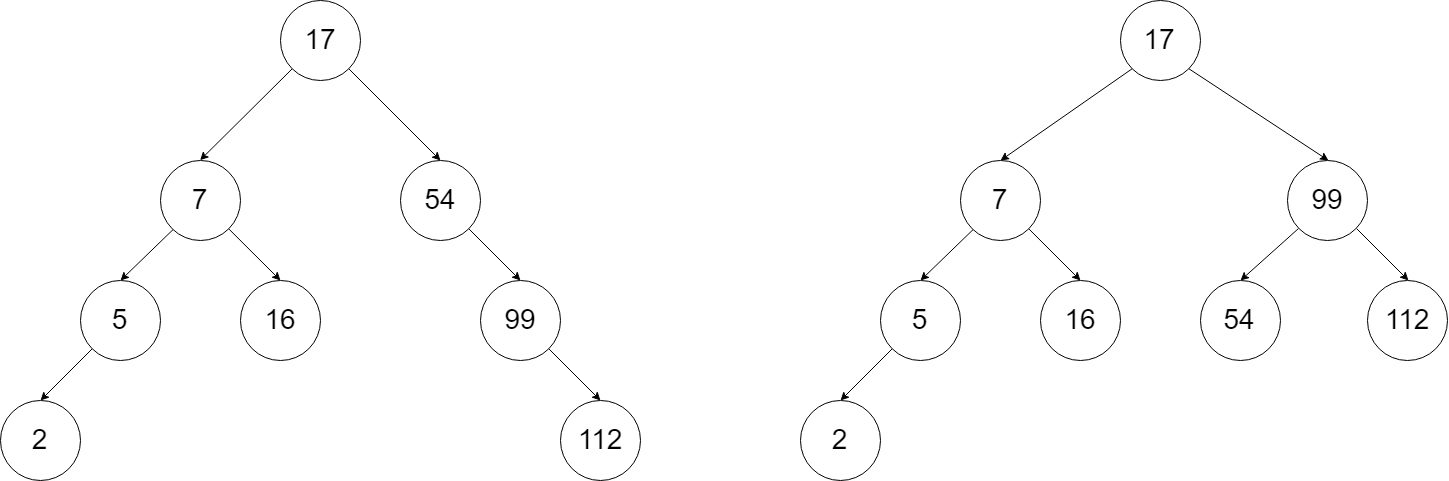
\includegraphics[width=\textwidth]{graph/avl_tree_visualized}
	\end{figure}
\end{frame}

\begin{frame}{Einfügen}{In AVL Bäume (Vgl. \cite{mutzel:avl}, \cite{wiki:avl})}
	\begin{itemize}
		\item Einfügen erfolgt vorerst nach normalem Verfahren von binären Suchbäumen
		\item Dadurch kann jedoch die AVL-Bedingung verletzt werden
		\item Dann muss der Baum wieder ausgeglichen werden
		\item Hierfür wird folgendermaßen vorgegangen:
		\begin{itemize}
			\item Wandere beginnend vo eingefügten Element $w$ nach oben
			\item Prüfe für jeden Knoten ob die AVL Bedingung verletzt ist
			\item Wenn ein Knoten $z$ gefunden wurde, für den die AVL-Bedingung verletzt wurde, gleiche den Baum aus
		\end{itemize}
	\end{itemize}
\end{frame}

\begin{frame}{Einfügen}{Ausgleichen von AVL Bäumen (vgl. \cite{avltree}, \cite{wiki:avl})}
	\begin{itemize}
		\item Zum Ausgleichen von AVL-Bäumen gibt des die Links- bzw. Rechtsrotation
		\item Für einen unbalancierten Knoten $x$ sei:
		\begin{itemize}
			\item $y$ Der "`Kindknoten"' (Erste schritt) von $x$ auf dem Weg zum eingefügten Knoten $w$
			\item $z$ Der "`Enkelknoten"' (Zweite Schritt) von $x$ auf dem Weg zu $w$
		\end{itemize}
		\item Hier gibt es vier mögliche Fälle nach denen unterschiedlich rotiert werden muss:
		\begin{itemize}
			\item Links-Links
			\item Links-Rechts
			\item Rechts-Rechts
			\item Rechts-Links
		\end{itemize}
	\end{itemize}
\end{frame}

\begin{frame}{Links-Links}{Rechtsrotation (Vgl. \cite{avltree})}
\begin{figure}
	\centering
	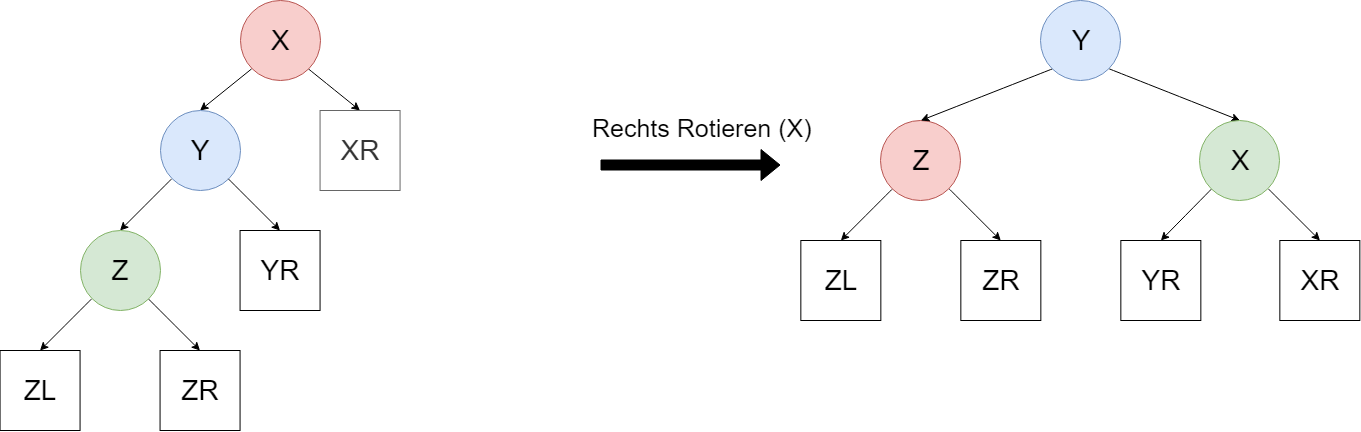
\includegraphics[width=\textwidth]{graph/avl_insert_ll}
\end{figure}
\end{frame}

\begin{frame}[allowframebreaks]{Links-Links}{Konkretes Beispiel}
\begin{figure}[ht!]
	\centering
	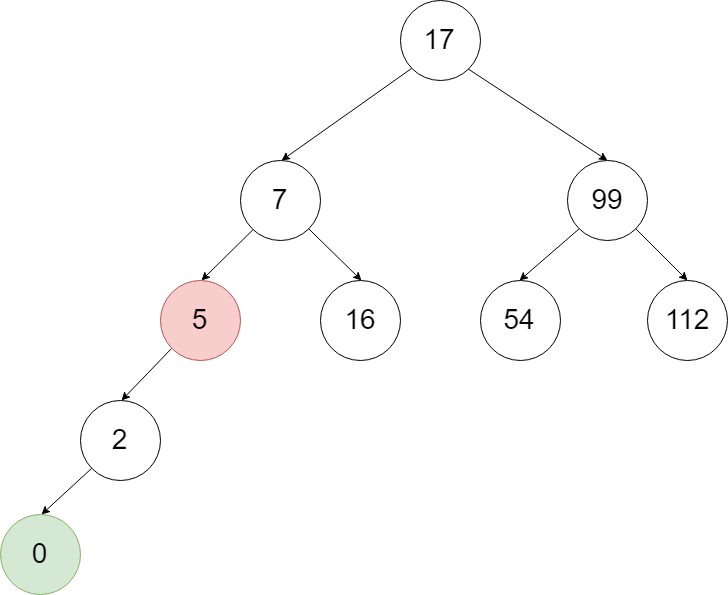
\includegraphics[height=5cm]{graph/avl_insert_ll_1}
\end{figure}
\framebreak
\begin{figure}
	\centering
	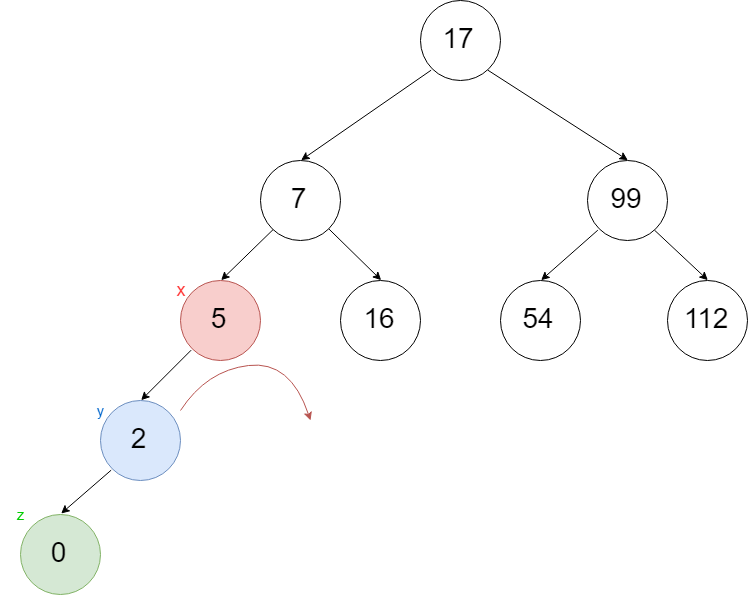
\includegraphics[height=6cm]{graph/avl_insert_ll_2}
\end{figure}
\framebreak
\begin{figure}
	\centering
	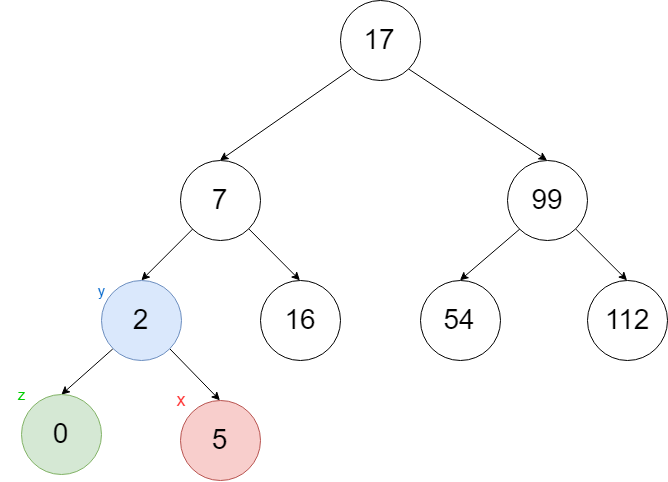
\includegraphics[height=6cm]{graph/avl_insert_ll_3}
\end{figure}

\end{frame}

\begin{frame}{Rechts-Rechts}{Linksrotation(Vgl. \cite{avltree})}
\begin{figure}
	\centering
	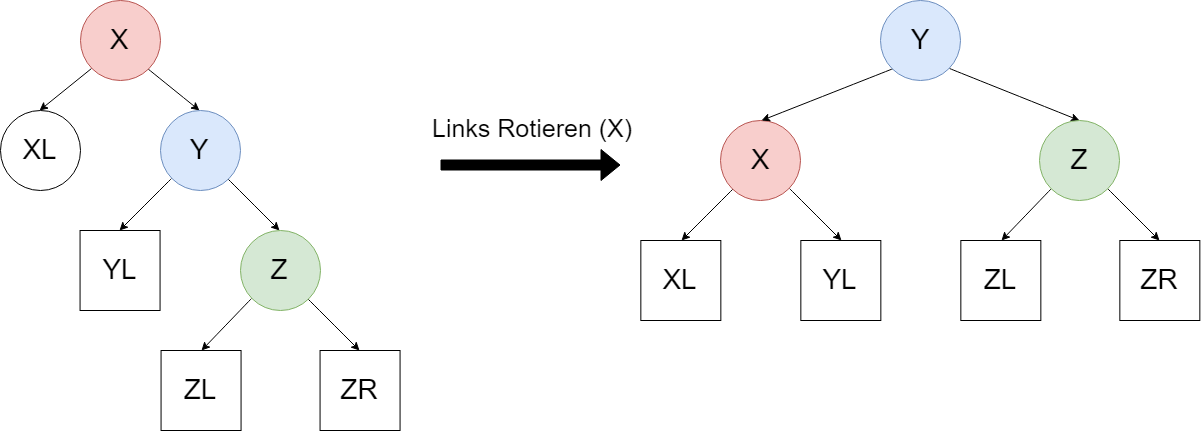
\includegraphics[width=\textwidth]{graph/avl_insert_rr}
\end{figure}
\end{frame}

\begin{frame}[allowframebreaks]{Rechts-Rechts}{Konkretes Beispiel}
\begin{figure}[ht!]
	\centering
	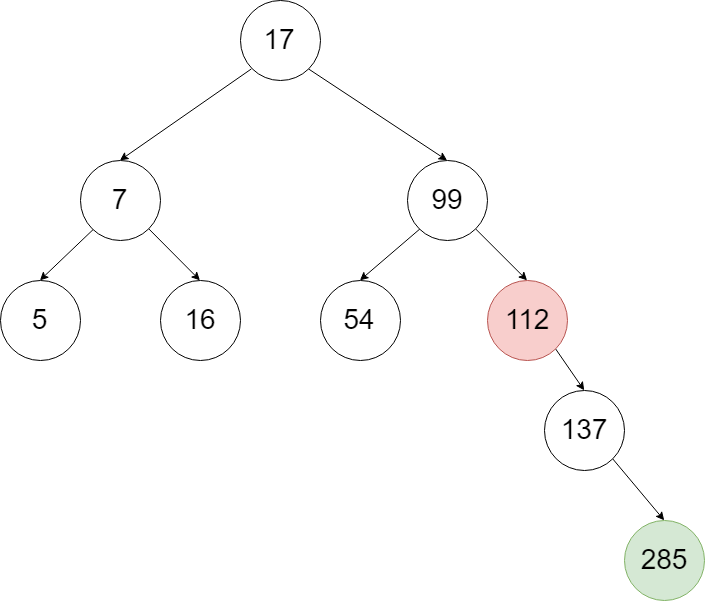
\includegraphics[height=5cm]{graph/avl_insert_rr_1}
\end{figure}
\framebreak
\begin{figure}
	\centering
	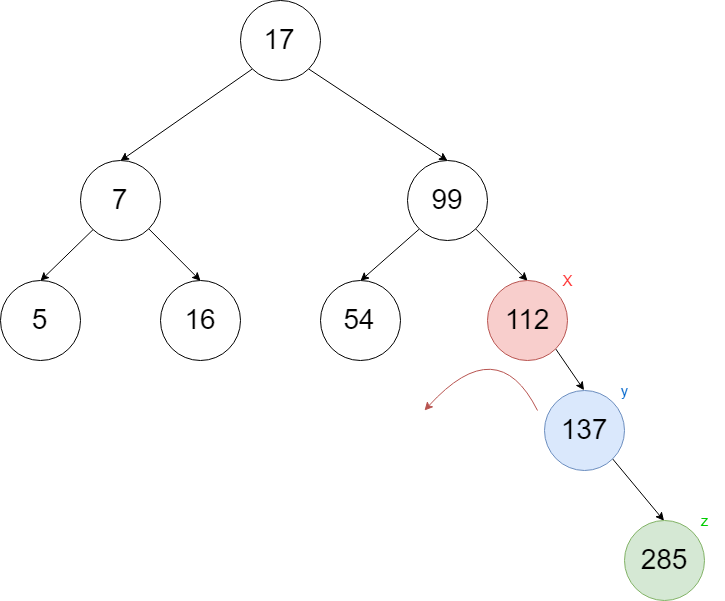
\includegraphics[height=6cm]{graph/avl_insert_rr_2}
\end{figure}
\framebreak
\begin{figure}
	\centering
	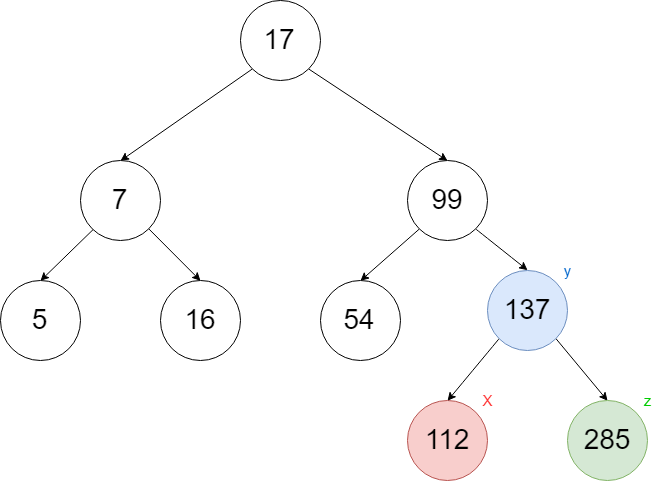
\includegraphics[height=6cm]{graph/avl_insert_rr_3}
\end{figure}

\end{frame}

\begin{frame}{Links-Rechts}{Links-Rechts-Doppelrotation(Vgl. \cite{avltree})}
\begin{figure}
	\centering
	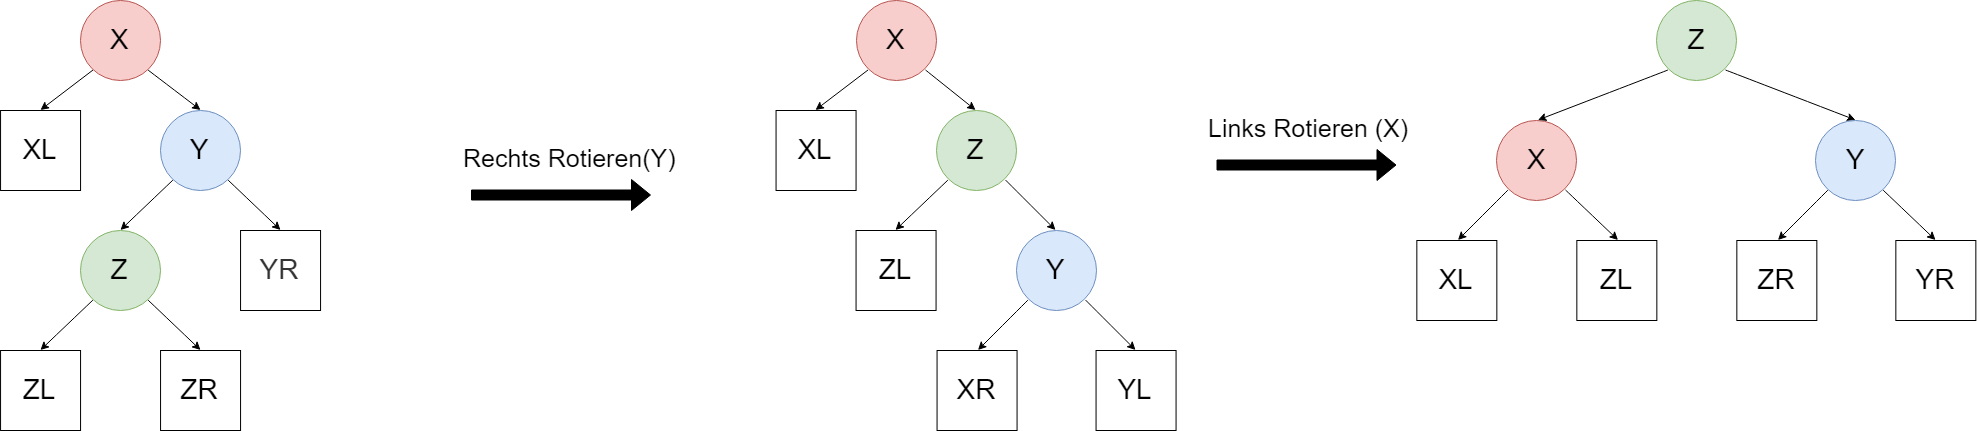
\includegraphics[width=\textwidth]{graph/avl_insert_rl}
\end{figure}
\end{frame}

\begin{frame}[allowframebreaks]{Links-Rechts}{Konkretes Beispiel}
\begin{figure}[ht!]
	\centering
	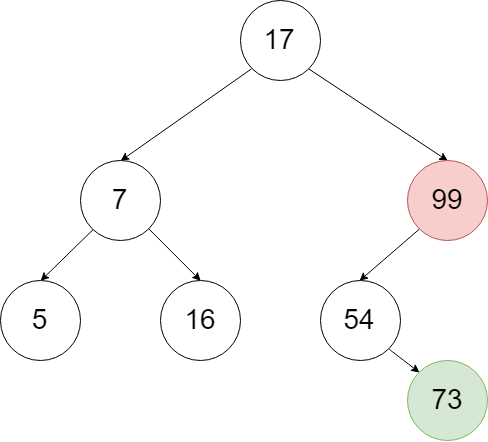
\includegraphics[height=5cm]{graph/avl_insert_lr_1}
\end{figure}
\framebreak
\begin{figure}
	\centering
	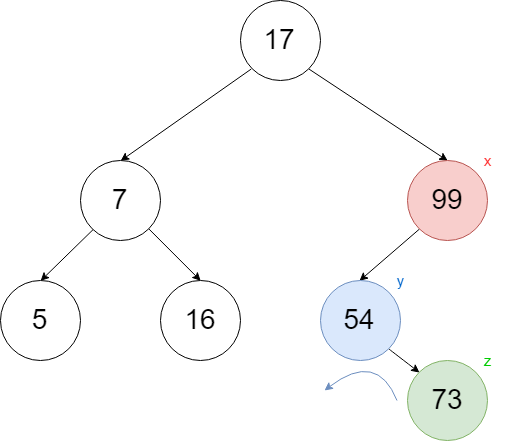
\includegraphics[height=6cm]{graph/avl_insert_lr_2}
\end{figure}
\framebreak
\begin{figure}
	\centering
	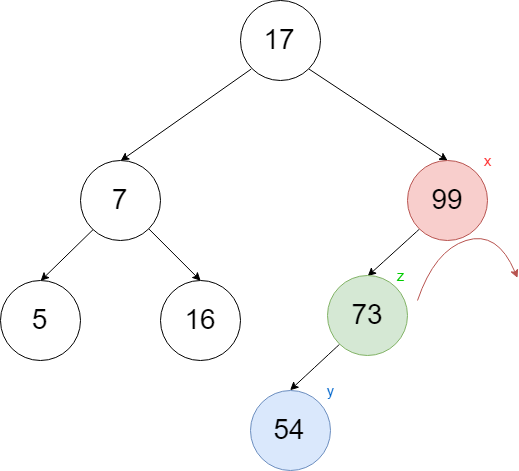
\includegraphics[height=6cm]{graph/avl_insert_lr_3}
\end{figure}
\framebreak
\begin{figure}
	\centering
	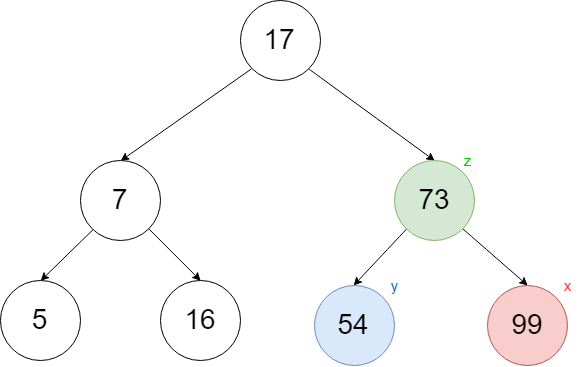
\includegraphics[height=6cm]{graph/avl_insert_lr_4}
\end{figure}

\end{frame}

\begin{frame}{Rechts-Links}{Rechts-Links-Doppelrotation (Vgl. \cite{avltree})}
\begin{figure}[ht!]
	\centering
	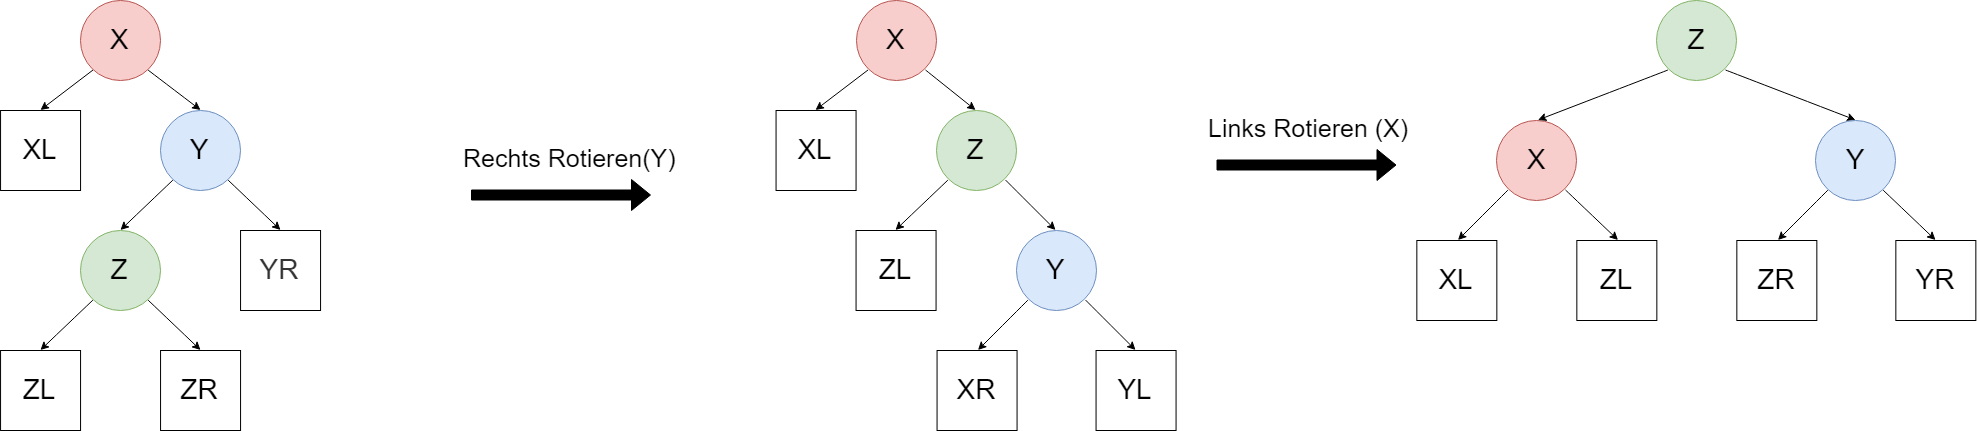
\includegraphics[width=\textwidth]{graph/avl_insert_rl}
\end{figure}
\end{frame}

\begin{frame}[allowframebreaks]{Rechts-Links}{Konkretes Beispiel}
\begin{figure}
	\centering
	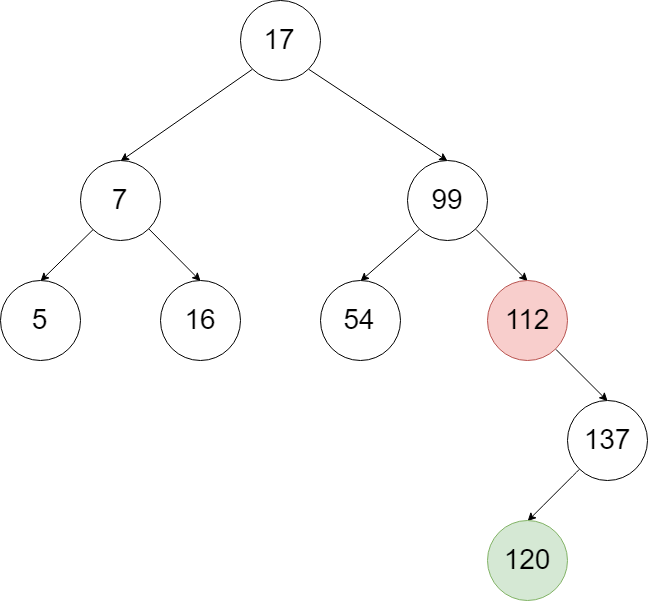
\includegraphics[height=5cm]{graph/avl_insert_rl_1}
\end{figure}
\framebreak
\begin{figure}
	\centering
	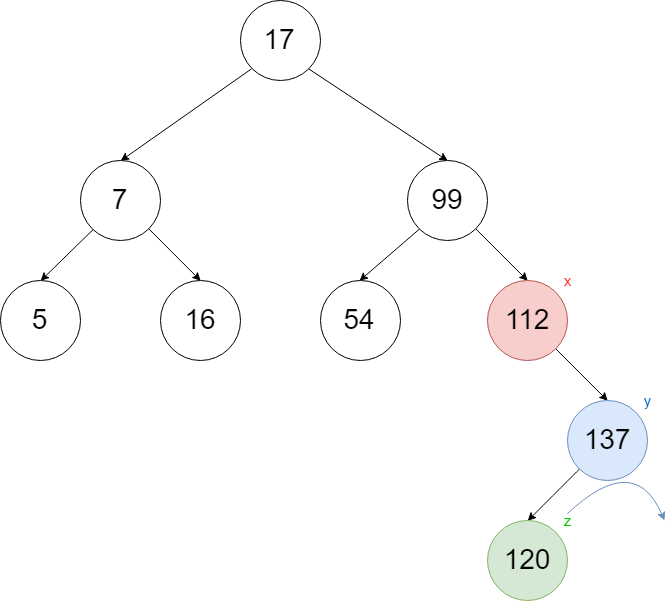
\includegraphics[height=6cm]{graph/avl_insert_rl_2}
\end{figure}
\framebreak
\begin{figure}
	\centering
	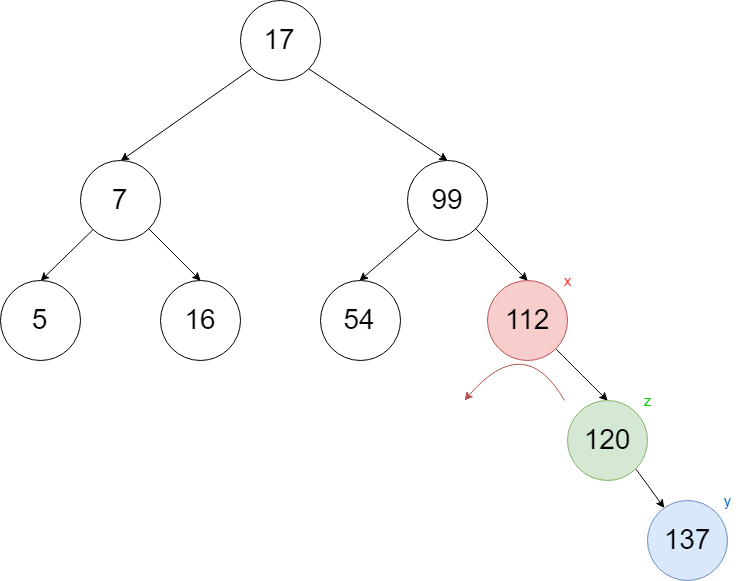
\includegraphics[height=6cm]{graph/avl_insert_rl_3}
\end{figure}
\framebreak
\begin{figure}
	\centering
	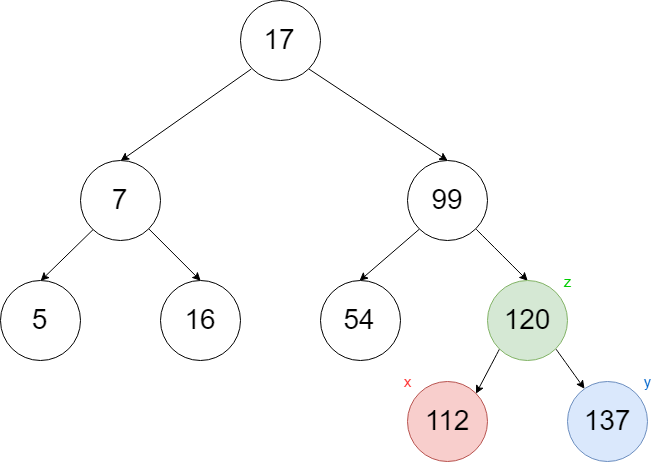
\includegraphics[height=6cm]{graph/avl_insert_rl_4}
\end{figure}

\end{frame}